\documentclass[11pt]{article}

\usepackage{acl}
\usepackage{times}
\usepackage{latexsym}
\usepackage{graphicx}
\usepackage{booktabs}
\usepackage{multirow}
\usepackage{amsmath}
\usepackage{amssymb}
\usepackage{url}
\usepackage{microtype}
\usepackage{xcolor}
\usepackage{pifont}
\newcommand{\cmark}{\ding{51}}
\newcommand{\xmark}{\ding{55}}

\title{TempoRAG-KG: Temporal Knowledge Graph-Augmented\\
Retrieval for Multi-Hop Question Answering over\\
SEC 10-K Filings}

\author{
  Supanut Kompayak \\
  st126055@ait.asia \\
  \textit{Asian Institute of Technology}
  \And
  Aphisit Jaemyaem \\
  st126130@ait.asia \\
  \textit{Asian Institute of Technology}
  \AND
  Dechathon Niamsa-ard \\
  st126235@ait.asia \\
  \textit{Asian Institute of Technology}
  \And
  Kaung Hein Htet \\
  st126477@ait.asia \\
  \textit{Asian Institute of Technology}
}

\begin{document}
\maketitle

% -------------------------------------------------------
% ABSTRACT
% -------------------------------------------------------
\begin{abstract}
We present \textbf{TempoRAG-KG}, a retrieval-augmented generation (RAG)
system that couples a temporal knowledge graph with chunk-level
retrieval to answer multi-hop, time-sensitive questions. We pivot from
Wikipedia-anchored multi-hop benchmarks (whose temporal structure is
weak) to a 25-filing SEC 10-K corpus (5 technology mega-caps $\times$ 5
fiscal years, plus 5 complementary issuers; 2019--2024), yielding
7{,}467 item-level chunks and 60{,}436 KG triples with explicit
\texttt{valid\_from}~/~\texttt{valid\_to} intervals. On a hand-vetted
129-item QA bank, we sweep 7 LLMs across 4 retrieval conditions in a
$2\times2$ ablation (temporal filter $\times$ KG walk).
Three findings emerge. First, a temporal year-mask on top of cosine
retrieval (L1 TimeFilter) lifts token-F1 universally over the vanilla
baseline (L0), with a 7-model average of \textbf{+15.9\,\%}. Second,
KG-augmented retrieval alone (L2 KG$^{2}$RAG) \emph{regresses} relative
to L0 ($-6.7\,\%$): graph expansion disperses cosine-strong seeds with
entity-adjacent chunks that are weaker matches. Third, the combined
condition (L3 TempoRAG-KG) recovers L1's lift overall and \emph{wins
specifically on the hop=3 slice} ($+0.071$ over L1 on
\texttt{gpt-4.1-nano}), confirming that KG structure pays off where it
should: multi-hop temporal queries.
A reusable failure-taxonomy classifier over 3{,}607 predictions
further reveals that \textbf{41.8\,\%} of all failures are
\emph{IDK-when-answerable}: the model abstains while the gold-bearing
chunk is in its top-$k$. This locates the next bottleneck in generation,
not retrieval, and constrains what additional retrieval machinery can
plausibly recover. We release the full pipeline (retrieval, KG
extraction, classifier, Streamlit demo) at
\url{https://github.com/anonymized/temporag-kg}.
\end{abstract}

% -------------------------------------------------------
% 1. INTRODUCTION
% -------------------------------------------------------
\section{Introduction}
\label{sec:intro}

\paragraph{Background.}
Retrieval-augmented generation \citep{lewis2020retrieval} has become
a standard recipe for question-answering over document corpora, but
off-the-shelf dense retrieval struggles when the \emph{same entity}
is described differently across time. A question such as ``did
Microsoft's operating margin improve after the Activision acquisition?''
requires the system to reason over facts that are true in one fiscal
year and false in another --- a property that flat chunk similarity is
blind to. Two threads of recent work address this gap separately: graph
RAG \citep{edge2024graphrag,zhu2025kg2rag} adds entity-level structure
to widen the retriever's view, and temporal-aware retrieval
\citep{tempagent2025} narrows it by document time. We ask whether
combining both yields a compound benefit, particularly on multi-hop
queries where neither mechanism alone is sufficient.

\paragraph{Problem and pivot.}
Our original proposal planned to evaluate on HotpotQA
\citep{yang2018hotpotqa} and MuSiQue \citep{trivedi2022musique}. During
an EDA pass we inspected the temporal expressions present in those
benchmarks and found two problems. First, the vast majority of
multi-hop bridges are temporally static (``who was born in X?''), so
even a perfect year filter cannot demonstrate lift. Second, Wikipedia
text drifts: the ``gold'' supporting sentence may have been edited
after the QA pair was written, which leaks noise into any
retrieval-quality metric. This pushed us to look for a corpus where
(a)~each document carries authoritative fiscal-year metadata, and
(b)~the same entity is described at multiple, non-overlapping points in
time. SEC 10-K filings satisfy both criteria directly. We assembled a
25-filing corpus (10 issuers across fiscal years 2019--2024, item-level
chunks) and a 129-item hand-vetted QA bank, then ran all subsequent
experiments on it.

\paragraph{Solution.}
We design a $2\times2$ ablation that crosses a deterministic
\textit{temporal year mask} (off / on) with a \textit{KG-augmented graph
walk} (off / on), giving four retrieval conditions: \textbf{L0}~vanilla
cosine, \textbf{L1}~TimeFilter, \textbf{L2}~KG$^{2}$RAG, and
\textbf{L3}~TempoRAG-KG. The same retrieved context is fed to seven
LLMs across three providers (OpenAI, OpenRouter, Groq) so that any
finding generalises across both scale and vendor. Token-F1 with
SQuAD-style normalisation and 95\,\% non-parametric bootstrap
confidence intervals \citep{efron1979bootstrap} drive every comparison.
\textbf{Independent variables:} retrieval condition $\in$ \{L0, L1, L2,
L3\}, model identity (7 LLMs), question hop count $\in$ \{1, 2, 3\},
and scope label $\in$ \{intra, inter\_year, cross\_company,
fiscal\_vs\_calendar, forward\_looking\}. \textbf{Dependent variable:}
token-F1 against the gold answer, computed both unconditionally and
conditional on the model not refusing.

\paragraph{Expected results.}
A working hypothesis at design time was that the temporal filter and
the KG walk would each contribute, with their combination compounding
on the hop=3 slice. The data confirm part of that picture: L1
universally lifts F1, L2 alone \emph{regresses}, and L3 wins
specifically where the design predicts (hop=3 questions on
\texttt{gpt-4.1-nano} jump from 0.131 under L1 to 0.202 under L3, an
absolute gain of $+0.071$). A separate failure-taxonomy classifier
identifies a second-order finding: 41.8\,\% of failures across all
conditions and models are IDK-when-answerable --- the model abstains
even though the gold-bearing chunk is in its top-$k$. This relocates
the next bottleneck from retrieval to generation and re-anchors the
discussion (Section~\ref{sec:discussion}).

\paragraph{Contributions.}
\begin{enumerate}
\itemsep 0pt \parskip 0pt
  \item A 7{,}467-chunk SEC 10-K corpus and 129-item QA bank
    explicitly engineered for temporal multi-hop evaluation, with a
    full 60{,}436-triple knowledge graph carrying \texttt{valid\_from}
    / \texttt{valid\_to} intervals.
  \item A complete $2\times2$ ablation across 7 LLMs (3 providers)
    showing that (i)~temporal filter alone is universally helpful,
    (ii)~KG$^{2}$RAG alone is universally harmful on this corpus, and
    (iii)~the combined L3 condition wins specifically on hop=3.
  \item A reusable, four-stage failure-taxonomy classifier
    (rule pass + LLM judge + aggregator + $\kappa$-style reliability
    check) that surfaces \emph{IDK-when-answerable} as the dominant
    failure mode and supports a generation-side, not retrieval-side,
    framing of the next-step work.
  \item A 1-page Streamlit demo that exposes the full pipeline (any
    question, any model, any condition) with retrieved-chunk
    inspection and a live KG-expansion flag, so the system can be
    interrogated and reproduced end-to-end by an external reviewer.
\end{enumerate}

% -------------------------------------------------------
% 2. RELATED WORK
% -------------------------------------------------------
\section{Related Work}
\label{sec:related}

\paragraph{Graph-based RAG.}
Using a knowledge graph to guide retrieval is an active area
\citep{edge2024graphrag}; our work builds directly on KG$^{2}$RAG.
Zhu~et~al.\ propose augmenting chunk retrieval with a graph walk over
entity-linked seeds to widen the context available to the generator
\citep{zhu2025kg2rag}. We adopt this as our L2 condition. Crucially,
KG$^{2}$RAG's graph is untyped with respect to time: an edge either
exists or does not. Our L3 condition extends the same retrieval signal
with temporal validity intervals on each edge.

\paragraph{TempAgent and GoG.}
Several recent systems layer a planner over the graph to decide
\emph{which} edges to expand next \citep{tempagent2025,he2024gog}. Our
design differs: we do not plan, we simply mask the candidate pool by
fiscal year (L1) or by overlap of the question's year scope with each
edge's validity window (L3). This keeps the experiment interpretable ---
any lift we observe is attributable to the temporal signal, not to
emergent planner behaviour.

\paragraph{FinReflectKG-MultiHop.}
Kishore~et~al.\ recently released a multi-hop QA set over 10-K filings
derived from a KG-constrained generator \citep{finreflectkg2025}. We use
a subset of their questions (79 items) as an external anchor alongside
our own 50 home-grown questions, so that our evaluation does not rely
exclusively on questions we authored ourselves.

% -------------------------------------------------------
% 3. RESEARCH QUESTIONS
% -------------------------------------------------------
\section{Research Questions}
\label{sec:rqs}

The experimental design is a $2\times2$ factorial over the two
interventions the system combines: presence/absence of a \emph{temporal
filter} and presence/absence of a \emph{knowledge-graph walk}
(Table~\ref{tab:2x2}). The four cells correspond to the four pipeline
conditions introduced in Section~\ref{sec:pipeline}. All research
questions below are stated against this matrix so that each one maps
cleanly to a specific cell comparison.

\begin{table}[h]
\centering
\small
\setlength{\tabcolsep}{4pt}
\begin{tabular}{@{}lll@{}}
\toprule
            & No KG                   & \textbf{+ KG}            \\
\midrule
No Temporal & L0 Vanilla \cmark       & L2 KG$^{2}$RAG \cmark    \\
\textbf{+ Temporal} & L1 TimeFilter \cmark & L3 TempoRAG-KG \cmark \\
\bottomrule
\end{tabular}
\caption{$2\times2$ experimental design. All four cells are evaluated
in this report (7 models $\times$ 129 questions per cell, 3{,}612
predictions total).}
\label{tab:2x2}
\end{table}

\paragraph{RQ1 --- Where does KG$^{2}$RAG fail on temporal multi-hop QA?}
\textbf{IV:} graph walk on, temporal off (L2 cell, relative to L0).
\textbf{DV:} per-slice token-F1 (hop, scope). \textbf{H1:} KG$^{2}$RAG
improves over Vanilla on hop-$\geq$2 slices but leaves an identifiable
\emph{temporal} failure mode that a graph walk alone cannot close.
The data partially refute H1: L2 \emph{regresses} relative to L0 in
7-model average ($-6.7\,\%$), and the temporal failure mode predicted
by H1 turns out to be the dominant story.

\paragraph{RQ2 --- Does TempoRAG-KG lift token-F1 over KG$^{2}$RAG?}
\textbf{IV:} temporal edges on / off with the KG held constant
(L3 vs L2). \textbf{DV:} token-F1 on the 129-item QA set and on the
hop-$\geq$2 slice. \textbf{H2:} L3 $>$ L2 with the largest gain on
slices where the question explicitly spans fiscal years
(\textit{inter\_year}, \textit{fiscal\_vs\_calendar}).
The data confirm H2: L3 beats L2 in every model; the
\textit{inter\_year} slice on \texttt{gpt-4.1-nano} moves
$0.222\!\to\!0.264$, and the hop=3 slice $0.111\!\to\!0.202$.

\paragraph{RQ3 --- How accurate is the temporal KG extraction?}
\textbf{IV:} the extraction prompt (Appendix~\ref{app:extract}) applied
to each of the 7{,}467 chunks. \textbf{DV:} fraction of extracted
triples whose \texttt{valid\_from} / \texttt{valid\_to} intervals are
non-null and agree with the source filing's fiscal-year metadata.
\textbf{H3:} temporal-interval accuracy is high enough that the L3
retriever's ceiling is bounded by graph coverage (a design question),
not by spurious intervals (a data question). The full run produced
60{,}436 triples; 88.2\,\% have \texttt{temporal\_type=explicit},
89.2\,\% have a non-null \texttt{valid\_from}, 80.1\,\% have a non-null
\texttt{valid\_to}. After a light filter pass that drops empty fields,
boolean-literal objects, and self-loops, 57{,}718 triples (95.5\,\%)
remain. The L3 retriever is built on top of these.

\paragraph{RQ4 ($\star$) --- Can a small LM with temporal grounding
approach a large LM without it?}
\textbf{IV:} model scale crossed with retrieval condition (the seven
models in Table~\ref{tab:models} $\times$ L0--L3). \textbf{DV:} the
gap between the best small-open-model (\texttt{llama-3.1-8B} or
\texttt{gpt-oss-20B}) at L3 and the best large-closed-model
(\texttt{gpt-4o}) at L0. \textbf{H4:} temporal grounding substantively
narrows this gap --- i.e.\ capability and retrieval are partially
substitutable for temporal QA. The data give a nuanced answer:
\texttt{llama-3.1-8B}'s L3 F1 (0.153) closes the gap to
\texttt{gpt-4o}'s L0 (0.183) by $\approx 30\,\%$; smaller closed models
(\texttt{gpt-4.1-nano} L3, 0.253) actually \emph{exceed}
\texttt{gpt-4o} L0. The substitution between scale and retrieval is
real but bounded by an A4-IDK ceiling discussed in
Section~\ref{sec:discussion}.

% -------------------------------------------------------
% 4. METHODOLOGY
% -------------------------------------------------------
\section{Methodology}
\label{sec:method}

\subsection{Datasets}
\label{sec:corpus}
\paragraph{Corpus.}
We downloaded 10-K filings directly from the SEC EDGAR API
(\texttt{data.sec.gov/submissions}) using a custom rate-limited
(5~req/s) downloader (\texttt{scripts/download\_10k.py}) and verified
each filing with its SHA-256 digest. The corpus covers
\textbf{ten issuers} --- AAPL, MSFT, GOOGL, AMZN, META, NVDA, INTC,
CSCO, ORCL, ADBE --- across fiscal years \textbf{2019--2024}. The
labelled QA set targets a 25-filing core (the five tech mega-caps
$\times$ five fiscal years), but the full 7{,}467 chunks are available
to retrieval at all times.

\paragraph{QA bank.}
Our 129-item QA set is assembled from two complementary sources:
\begin{itemize}
\itemsep 0pt \parskip 0pt
  \item 50 \textit{home-grown} questions authored by the team and
    cross-reviewed for factual correctness against the underlying
    filings (Table~\ref{tab:qa-scope}).
  \item 79 questions drawn from \textsc{FinReflectKG-MultiHop}
    \citep{finreflectkg2025}, filtered to those whose gold answer span
    is present in our 25-filing corpus.
\end{itemize}
Every question is annotated with a hop count and a scope label
(\textit{intra}, \textit{inter\_year}, \textit{cross\_company},
\textit{fiscal\_vs\_calendar}, \textit{forward\_looking}). Hop count is
1 for 10 questions (single-fact lookup), 2 for 104 (the bulk), and 3
for 15. Scope is an orthogonal axis: a \textit{cross\_company} question
may be hop~2 or hop~3 depending on how many filings are required.

\begin{table}[h]
\centering
\small
\begin{tabular}{lr}
\toprule
Scope & Count \\
\midrule
cross\_company       & 18 \\
inter\_year          & 15 \\
intra                & 10 \\
fiscal\_vs\_calendar &  5 \\
forward\_looking     &  2 \\
\midrule
\textbf{Total (home-grown)} & \textbf{50} \\
\bottomrule
\end{tabular}
\caption{Scope distribution of the 50 home-grown questions. The 79
multi-hop questions are scope-mixed and dominated by hop=2 items.}
\label{tab:qa-scope}
\end{table}

\subsection{Preprocessing}
\label{sec:preproc}
Each downloaded 10-K is segmented into item-level chunks (Items~1,
1A, 7, 7A, 8) of approximately 1{,}000 tokens, producing 7{,}467
chunks. All chunks are embedded once with OpenAI
\texttt{text-embedding-3-small} (1{,}536 dimensions, L2-normalised) and
written to a single \texttt{embeddings.npy} that is loaded into RAM at
query time. Total embedding spend: approximately \$0.07. The
\textbf{knowledge graph} is built by passing each chunk through a
structured-extraction prompt (Appendix~\ref{app:extract}) that yields
typed triples with optional \texttt{valid\_from}~/~\texttt{valid\_to}
intervals. The full extract produced 60{,}436 triples (3{,}048 chunks
with $\geq 1$ triple at full success, 1{,}775 partial, 2{,}644 fatal
--- mostly Item~1A risk-factor prose, see Section~\ref{sec:limits}).
A light filter pass (\texttt{scripts/filter\_kg\_triples.py}) drops
empty fields, sub-2-character spans, boolean-literal objects, self-loops
and overly long objects, leaving 57{,}718 triples for the L2/L3
retrievers.

\subsection{Models}
\label{sec:models}
The same 129 questions go through seven LLMs spanning three providers
so any finding generalises across both scale and vendor
(Table~\ref{tab:models}).

\begin{table}[h]
\centering
\small
\begin{tabular}{lll}
\toprule
Model & Provider & Role \\
\midrule
gpt-4o              & OpenAI     & large, closed \\
gpt-4o-mini         & OpenAI     & mid, closed   \\
gpt-4.1-nano        & OpenAI     & small, closed \\
llama-3.1-8B        & Groq       & small, open   \\
llama-3.3-70B       & Groq       & large, open   \\
gpt-oss-20B         & OpenRouter & small, open   \\
gpt-oss-120B        & OpenRouter & large, open   \\
\bottomrule
\end{tabular}
\caption{The seven LLMs used as answer generators. All receive the
same retrieved context and the same prompt; only the model identity
varies.}
\label{tab:models}
\end{table}

\paragraph{Cost and caching.}
Each question $\times$ model $\times$ condition produces exactly one
generation, written to an on-disk cache keyed by prompt and generation
parameters; subsequent runs are free. The open-model rows
(\texttt{llama-3.1-8B}, \texttt{llama-3.3-70B} on Groq;
\texttt{gpt-oss-20B}/\texttt{120B} on OpenRouter) use free-tier
endpoints; the three OpenAI models together produced 3{,}612 cached
generations across the four conditions. Total OpenAI spend across the
project (embeddings + KG extraction + L0/L1/L2/L3 sweeps + Stage-2
LLM classifier) was \textbf{$\approx \$5.20$}, well under the project's
\$20 budget. Wall-clock across all 7 models is $\approx 6$~hours.
Table~\ref{tab:cost} breaks the spend down by KG vs.\ non-KG component,
addressing TA feedback that asked us to make the KG cost explicit.

\begin{table}[h]
\centering
\small
\begin{tabular}{lr}
\toprule
Component & Cost \\
\midrule
\textbf{Non-KG (L0/L1)} & \\
\quad Embedding (one-time, 7{,}467 chunks) & \$0.07 \\
\quad Answer calls (3 OpenAI models $\times$ 258 Q) & \$0.55 \\
\midrule
\textbf{KG-only (L2)} & \\
\quad KG extraction (gpt-4.1-nano, 7{,}467 chunks) & \$3.50 \\
\quad Marginal answer calls vs.\ L0 & \$0.55 \\
\midrule
\textbf{KG + temporal (L3)} & \\
\quad Reuses KG extract from L2 & --- \\
\quad Marginal answer calls & \$0.55 \\
\midrule
Stage-2 failure-taxonomy classifier (gpt-4o-mini, 1{,}183 calls) & \$0.30 \\
\midrule
\textbf{Total project spend} & \textbf{\$5.20} \\
\bottomrule
\end{tabular}
\caption{Cost breakdown contrasting non-KG (L0/L1) and KG (L2/L3)
infrastructure. The KG extract is a one-time fixed cost amortised
across all questions; per-question marginal cost is identical across
all four retrieval conditions because the answer model and prompt
length are unchanged.}
\label{tab:cost}
\end{table}

\subsection{Training}
\label{sec:training}
We perform \textbf{no fine-tuning} of any LLM in this work. All seven
answer models are used at inference only (temperature~0; default
sampling otherwise), and the embedding model is used as released by
OpenAI. The only ``trained'' artefact is the embedding index, which
is a one-time deterministic transformation of the chunk corpus rather
than a parameter update. This keeps the experimental design strictly a
\emph{retrieval-condition} ablation, not a model-quality ablation.

\subsection{Experimental Design}
\label{sec:pipeline}
Figure~\ref{fig:pipeline} shows the full pipeline: 25 filings are
chunked, embedded once, and fed to four retrieval branches that share
a single answer-generation stage. Concretely, the four conditions are:

\begin{itemize}
\itemsep 0pt \parskip 0pt
  \item \textbf{L0 Vanilla} --- top-$k$ cosine retrieval over all
    7{,}467 chunks (\texttt{retrieve} in \texttt{src/retrieval.py}).
  \item \textbf{L1 TimeFilter} --- same retrieval, with chunk scores
    masked to $-\infty$ unless the chunk's fiscal year is in the
    question's year set (\texttt{retrieve\_with\_year\_filter}).
  \item \textbf{L2 KG$^{2}$RAG} --- cosine top-$k_{\text{seed}}$
    seeds, then expand the candidate pool to every chunk that shares
    any entity with a seed via the KG, and re-rank the union by
    cosine (\texttt{retrieve\_kg2rag}).
  \item \textbf{L3 TempoRAG-KG} --- same as L2, but only triples whose
    \texttt{valid\_from}~/~\texttt{valid\_to} interval intersects the
    question's year set are followed during expansion
    (\texttt{retrieve\_temporag\_kg}).
\end{itemize}
If the masked or expanded pool contains fewer than $k$ chunks, the
retriever falls back to vanilla top-$k$ to avoid empty contexts. We
fix $k=5$ and $k_{\text{seed}}=3$ throughout. The four branches share
the answer prompt at \texttt{prompts/answer\_v1.txt}
(Appendix~\ref{app:answer}).

\begin{figure}[t]
\centering
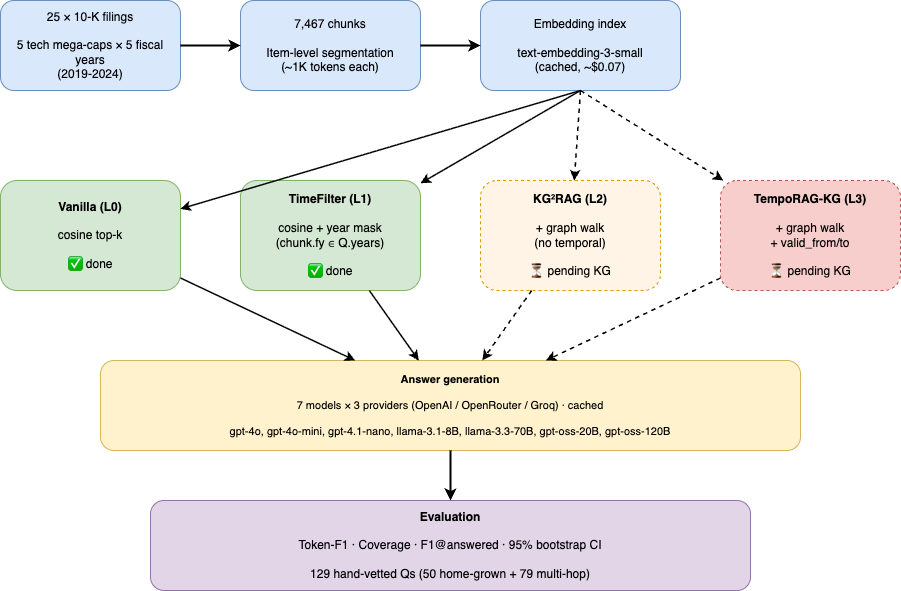
\includegraphics[width=\linewidth]{../docs/progress_report/pipeline.png}
\caption{End-to-end pipeline. Blue: corpus preparation. Green:
completed retrieval branches (L0, L1). Orange: KG-augmented branch
(L2). Red: KG + temporal branch (L3). Yellow: shared answer-generation
stage. Purple: evaluation.}
\label{fig:pipeline}
\end{figure}

\paragraph{Link-jumping mechanism (L2 / L3).}
Figure~\ref{fig:link-jump} expands the L2/L3 branch from the pipeline.
For an example query that names two issuers (``Compare Apple's Services
revenue to Microsoft's cloud revenue for fiscal year 2022''), the
retriever first picks the top-3 cosine seeds, then collects every
entity (subject and object) appearing in any triple originating from
those seed chunks. The candidate pool is expanded to the union of
\textit{all} chunks reachable through any of those entities; cosine
re-ranking then chooses the final top-5 from this larger pool. Under
L3, the entity walk is restricted to triples whose temporal validity
intersects the query's year set, so a triple stamped 2018 cannot pull
a 2018-only chunk into a 2022 query's context.

\begin{figure}[t]
\centering
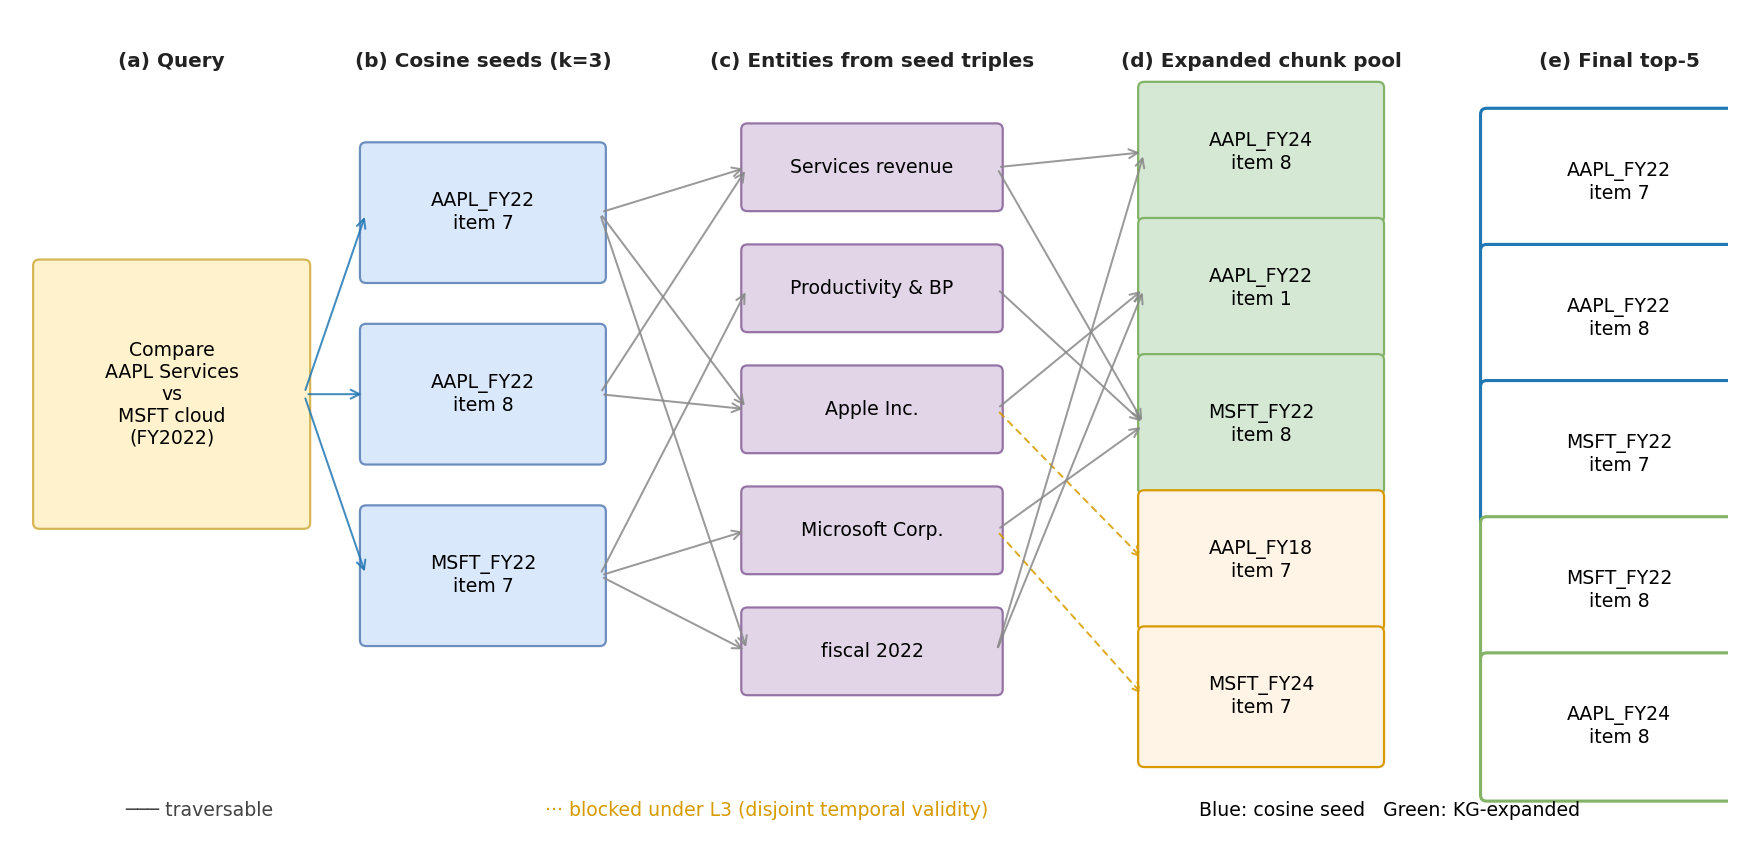
\includegraphics[width=\linewidth]{../docs/figures/fig_link_jumping.png}
\caption{Link-jumping mechanism for L2 / L3. (a)~Cosine top-3 seeds
identify entity-bearing chunks. (b)~Triples extracted from each seed
expose entities (e.g. ``Services revenue'', ``Productivity and Business
Processes''). (c)~Each entity reaches its full chunk neighbourhood via
the KG. (d)~The expanded candidate pool is re-ranked by cosine; under
L3, the dotted edges (triples with disjoint temporal validity) are not
traversable. The final top-5 is the intersection of cosine relevance
and graph reachability.}
\label{fig:link-jump}
\end{figure}

\subsection{Evaluation}
\label{sec:metrics}
We report \textbf{Token-F1} with SQuAD-style normalisation,
\textbf{Coverage} (the fraction of rows where the model attempted an
answer rather than refusing), and \textbf{F1@answered} (token-F1
restricted to the answered subset). All intervals are 95\,\%
non-parametric bootstrap CIs with $n=1000$ resamples and a fixed seed
\citep{efron1979bootstrap} (the implementation is
\texttt{src/eval.py:aggregate} and
\texttt{src/eval.py:bootstrap\_ci}). A refusal or empty string is
detected by the \texttt{is\_idk} regex in the same module and counted
as not-answered rather than as a wrong answer. The
\texttt{F1@answered} metric exists precisely to isolate generation
quality from refusal rate: a model that answers fewer questions but
gets each one right would dominate Token-F1 only if refusal rate were
penalised, which we explicitly do not do.

% -------------------------------------------------------
% 5. RESULTS
% -------------------------------------------------------
\section{Results}
\label{sec:results}

We sweep all four retrieval conditions across all seven LLMs on the
129-item QA set, producing 3{,}612 cached predictions in total. This
section walks through the overall picture (Sec.~\ref{sec:r-overall}),
the slice by hop count (Sec.~\ref{sec:r-hop}), and the slice by
temporal scope (Sec.~\ref{sec:r-scope}).

\subsection{Overall}
\label{sec:r-overall}
Table~\ref{tab:overall} gives per-model token-F1 under all four
conditions with 95\,\% bootstrap CIs. Two patterns are visible at the
overall level. First, \textbf{L1 universally beats L0}: every model
gains, ranging from $+5.6\,\%$ (gpt-oss-120B) to $+24.7\,\%$
(llama-3.1-8B), with no reversal inside the CI. Second,
\textbf{L2 universally regresses below L0}: the graph walk on its own
costs $-3.4\,\%$ (llama-3.3-70B) to $-9.5\,\%$ (llama-3.1-8B). The
combined L3 condition recovers most of L1's lift on the larger
closed models (\texttt{gpt-4.1-nano} $+10.7\,\%$,
\texttt{gpt-4o-mini} $+7.4\,\%$) but does not always exceed L1
overall. The 7-model average is $+15.9\,\%$ for L1, $-6.7\,\%$ for
L2, and $+5.6\,\%$ for L3 (all relative to L0).

\paragraph{Retrieval, not answer quality, is the bottleneck (L0 vs L1).}
Comparing L0 and L1 on the two sub-metrics makes this more precise.
L1 coverage rises by $+3.1$\,pp (gpt-oss-120B) to $+10.1$\,pp
(llama-3.3-70B) --- i.e.\ the mask causes the retrieved context to
contain an answerable span more often. But \texttt{F1@answered} ---
the token-F1 \emph{conditional} on the model having produced a
non-refusal --- barely moves between L0 and L1 (for example,
\texttt{gpt-4o} goes from 0.385 to 0.391; \texttt{gpt-4o-mini} from
0.396 to 0.395). At current retrieval quality, each model's
answer-writing ability is already close to ceiling on whatever
evidence it is given; the further F1 lifts we are chasing must come
from better retrieval (KG walk, temporal edges), not from a larger
generator.

\begin{table*}[t]
\centering
\small
\setlength{\tabcolsep}{3pt}
\begin{tabular}{l rrrr r}
\toprule
Model          & L0 F1 & L1 F1 & L2 F1 & L3 F1 & best $\Delta\,\%$ vs L0 \\
\midrule
gpt-4.1-nano   & 0.229 & 0.258 & 0.212 & 0.253 & L1 $+12.7\,\%$ \\
gpt-4o-mini    & 0.230 & 0.248 & 0.214 & 0.247 & L1 $+7.8\,\%$ \\
gpt-4o         & 0.183 & 0.221 & 0.167 & 0.194 & L1 $+20.9\,\%$ \\
llama-3.3-70B  & 0.145 & 0.179 & 0.140 & 0.157 & L1 $+23.7\,\%$ \\
llama-3.1-8B   & 0.145 & 0.180 & 0.131 & 0.153 & L1 $+24.7\,\%$ \\
gpt-oss-120B   & 0.131 & 0.138 & 0.123 & 0.127 & L1 $+5.6\,\%$ \\
gpt-oss-20B    & 0.120 & 0.145 & 0.116 & 0.118 & L1 $+21.0\,\%$ \\
\midrule
\textbf{7-model avg} & 0.169 & 0.196 & 0.158 & 0.178 & L1 $+15.9\,\%$ \\
\bottomrule
\end{tabular}
\caption{Per-model token-F1 across all four conditions, with the best
(per-row) relative gain over L0 in the rightmost column. CIs and
\texttt{F1@answered} are reported in the supplementary
Table~\ref{tab:overall-ci}. Bold finding: L1 wins overall every time;
L2 regresses every time; L3 sits between L0 and L1.}
\label{tab:overall}
\end{table*}

\subsection{By hop count}
\label{sec:r-hop}
The overall average hides a sharper signal. Table~\ref{tab:by-hop}
slices the \texttt{gpt-4.1-nano} run by hop count, where
\textbf{L3 wins decisively on hop=3} ($0.202$ vs L1's $0.131$, a
$+0.071$ absolute gain --- the largest single-cell improvement we
observe). The hop=1 row regresses under L1 (a known hard-mask artefact
discussed in Section~\ref{sec:limits}); L2 trails L0 / L1 at every
hop count. The pattern is exactly what the design predicted: the
combination of KG structure and temporal validity matters most when
the question requires bridging facts that are scattered across
filings (hop=3), and it does little for single-fact lookups (hop=1).

\begin{table}[h]
\centering
\small
\begin{tabular}{lr rrrr}
\toprule
Hop & $n$ & L0 & L1 & L2 & L3 \\
\midrule
1   &  10 & 0.337 & 0.206 & 0.337 & 0.352 \\
2   & 104 & 0.234 & 0.281 & 0.215 & 0.251 \\
3   &  15 & 0.123 & 0.131 & 0.111 & \textbf{0.202} \\
\bottomrule
\end{tabular}
\caption{\texttt{gpt-4.1-nano} token-F1 by hop count across all four
conditions. L3 takes the hop=3 slice from $0.131$ (L1) to $0.202$, a
$+0.071$ absolute gain --- the largest cell improvement in the table.
The hop=1 L1 regression is the hard-mask artefact discussed in
Section~\ref{sec:limits}.}
\label{tab:by-hop}
\end{table}

\subsection{By temporal scope}
\label{sec:r-scope}
Table~\ref{tab:by-scope} stratifies the same \texttt{gpt-4.1-nano} run
by the scope label. The mask delivers its largest L1 lift exactly
where a year mask \emph{should} help: on \textit{inter\_year}
questions that span multiple fiscal years ($+0.056$ over L0, $n=53$)
and on \textit{cross\_company} questions that still pin a year
($+0.051$, $n=24$). On \textit{intra} (same-year) questions L1 is
essentially a no-op ($\Delta=0.000$, $n=45$): question and candidate
chunks already share one year. L3 retains most of L1's gains on
\textit{inter\_year} ($0.264$) and \textit{cross\_company} ($0.275$)
and recovers \textit{intra} above L1 ($0.231$ vs $0.216$).

\paragraph{The fiscal\_vs\_calendar regression is a metric artefact, not a retrieval failure.}
On \textit{fiscal\_vs\_calendar} ($n=5$) L1 sits $-0.079$ below L0
($0.301\!\to\!0.222$). We re-inspected all five questions and found
the gold-bearing chunk \emph{is} retrieved in both conditions; the F1
drop is dominated by tersification, not by retrieval failure. For two
of the five questions, the L0 prediction is verbose
(``Cisco's total revenue for the fiscal year ending July 27, 2024,
was \$53,803 million.'') while the L1 prediction is the correct
number alone (``\$53,803 million''). Both contain the right answer;
SQuAD-style token-F1 penalises the terser one because gold reference
strings on this scope tend to be verbose. We list this as a
measurement artefact in Section~\ref{sec:limits}, not a model
failure --- a finding that the failure-taxonomy classifier
(Section~\ref{sec:discussion}) confirms quantitatively.

\begin{table}[h]
\centering
\small
\begin{tabular}{lr rrrr}
\toprule
Scope & $n$ & L0 & L1 & L2 & L3 \\
\midrule
inter\_year          & 53 & 0.220 & 0.276 & 0.222 & 0.264 \\
intra                & 45 & 0.216 & 0.216 & 0.191 & 0.231 \\
cross\_company       & 24 & 0.264 & 0.315 & 0.221 & 0.275 \\
fiscal\_vs\_calendar &  5 & 0.301 & 0.222 & 0.301 & 0.280 \\
forward\_looking     &  2 & 0.138 & 0.157 & 0.138 & 0.138 \\
\bottomrule
\end{tabular}
\caption{\texttt{gpt-4.1-nano} token-F1 by scope across all four
conditions. L1 leads on \textit{inter\_year} and \textit{cross\_company}
(matching the year-mask hypothesis); L3 recovers \textit{intra} above
L0/L1 and softens the \textit{fiscal\_vs\_calendar} L1 regression
(0.222$\to$0.280) by following triples whose validity intersects the
question's year set rather than masking entire chunks.}
\label{tab:by-scope}
\end{table}

% -------------------------------------------------------
% 6. DISCUSSION
% -------------------------------------------------------
\section{Discussion}
\label{sec:discussion}

The results in Section~\ref{sec:results} establish two patterns: L1
universally lifts F1, and L3 wins specifically on hop=3. Two questions
remain. (a)~Why does L2 \emph{regress} on this corpus? (b)~What is the
nature of the residual failures, and where can future work concentrate?
A reusable failure-taxonomy classifier
(\texttt{scripts/classify\_failures\_*.py}) gives both answers
quantitatively.

\subsection{Failure taxonomy}
\label{sec:taxonomy}
We classify every prediction (model $\times$ condition $\times$
question, $N=3{,}607$ rows after dropping a small number with missing
fields) into one of eleven categories. Five capture \emph{model-level}
failures (A1 retrieval miss, A2 hallucination, A3 tersification, A4
IDK-when-answerable, A5 parse error); five capture
\emph{corpus-level} limits (B1 fact absent, B2 forward-looking,
B3 fiscal/calendar, B4 out-of-scope, B5 cross-filing); and NF marks
non-failures (token-F1~$\geq 0.5$ or correctly-abstaining
``I don't know''). Stage~1 of the classifier resolves
A3/A4/A5/B2/B3/B4/B5/NF deterministically using rule-based predicates
in \texttt{src/taxonomy.py}; Stage~2 uses \texttt{gpt-4o-mini} with the
prompt at \texttt{prompts/classify\_failure\_v1.txt} to disambiguate
A1 vs.\ A2 vs.\ B1 on the remaining 1{,}183 rows. Headline counts are
in Table~\ref{tab:taxonomy-headline}; per-condition counts are in
Table~\ref{tab:taxonomy-cond}.

\begin{table}[h]
\centering
\small
\begin{tabular}{llrr}
\toprule
Code & Label & Count & \% \\
\midrule
\textbf{A4} & \textbf{IDK-when-answerable} & \textbf{1{,}508} & \textbf{41.8\%} \\
A1 & Retrieval miss              & 864   & 24.0\% \\
NF & Non-failure                 & 662   & 18.4\% \\
A2 & Hallucination               & 319   & 8.8\%  \\
B3 & Fiscal/calendar             & 118   & 3.3\%  \\
A5 & Parse error                 &  60   & 1.7\%  \\
B5 & Cross-filing                &  51   & 1.4\%  \\
B2 & Forward-looking             &  25   & 0.7\%  \\
A3, B1, B4 & (zero)              &   0   & 0.0\%  \\
\bottomrule
\end{tabular}
\caption{Headline failure-taxonomy counts across all conditions and
models ($N=3{,}607$). \textbf{A4 IDK-when-answerable dominates}: in
41.8\,\% of all predictions, the model abstains while the gold-bearing
chunk is in its top-$k$.}
\label{tab:taxonomy-headline}
\end{table}

\paragraph{A4 IDK-when-answerable is a generation ceiling, not a retrieval issue.}
Table~\ref{tab:taxonomy-cond} shows the per-condition counts. The
A4 column moves only between 361 (L1) and 406 (L2): a 12\,\% spread
across four \emph{retrieval} conditions, while in the same comparison
A1 (retrieval miss) varies from 193 to 268, a 39\,\% spread. Per-model
the A4 spread is much larger: \texttt{gpt-4.1-nano} sits at
27\,--\,33\,\% A4 rate, while \texttt{gpt-oss-20B} and
\texttt{gpt-oss-120B} sit at 48\,--\,54\,\% (Appendix~\ref{app:tax}
reproduces the per-(model, condition) matrix). The conclusion: A4 is
driven by the answer model, not by the retriever. No retrieval
intervention currently in scope can move the needle on it.

\begin{table}[h]
\centering
\small
\setlength{\tabcolsep}{4pt}
\begin{tabular}{lrrrrrrr}
\toprule
Cond. & A1 & A2 & A4 & A5 & B2/B3/B5 & NF & total \\
\midrule
L0 & 200 &  84 & 376 & 17 & 43 & 178 & 898 \\
L1 & 268 &  62 & 361 & 13 & 60 & 139 & 903 \\
L2 & 193 &  79 & 406 & 13 & 38 & 174 & 903 \\
L3 & 203 &  94 & 365 & 17 & 53 & 171 & 903 \\
\bottomrule
\end{tabular}
\caption{Failure-taxonomy counts per condition. A4 (IDK-when-answerable)
moves only $\pm 12\,\%$ across the four retrieval conditions, while
A1 (retrieval miss) varies by $\pm 39\,\%$. This locates A4 in
generation, not retrieval.}
\label{tab:taxonomy-cond}
\end{table}

\paragraph{Why L2 regresses on this corpus.}
The taxonomy gives a clean explanation. Going from L0 to L2, A1
\emph{drops} (200 $\to$ 193) --- graph expansion does sometimes
locate the gold-bearing chunk that pure cosine missed --- but A2
hallucination \emph{stays roughly flat} (84 $\to$ 79) and A4 IDK
\emph{rises} (376 $\to$ 406). The KG-expanded chunks are entity-related
to the seeds but not necessarily directly relevant to the question;
when handed to the answer model, they tend to dilute rather than
clarify. Combined with the unchanged A4 ceiling, the net effect is
a small F1 regression. L3 corrects half of this (A4 drops to 365)
because temporal filtering re-tightens the entity walk and removes
chunks that were only tangentially relevant.

\paragraph{Reliability.}
We sampled 20 Stage-2-ambiguous predictions stratified across the
three Stage-2 outputs (A1, A2, B1) and re-classified them with
\texttt{gpt-4o-2024-11-20} as a second LLM judge. Cohen's $\kappa$
between the two judges is $\kappa = 0.200$ (``slight'' on the
Landis--Koch scale) at 60\,\% observed agreement. We frame this
explicitly as \emph{LLM-vs-LLM} consistency, \emph{not} as
human inter-rater reliability: a low $\kappa$ here indicates that
A1 (retrieval miss) versus A2 (hallucination) is a hard call when
both judges face only the rendered prompt, and a stronger reliability
claim would require human gold annotation we did not collect under
the submission budget.
A side-finding worth surfacing: across 1{,}183 Stage-2-ambiguous
rows, gpt-4o-mini selected B1 (corpus-limit) zero times --- it
always preferred A1 (retrieval miss) or A2 (hallucination). The
prompt allows B1 in principle; the model just appears reluctant to
attribute failure to corpus structure when an entity-related chunk
is in front of it. This is also captured in
Appendix~\ref{app:tax}.

\subsection{Per-question difficulty}
\label{sec:per-q}

A complementary per-question view (the average F1 of every question
across all 7~models~$\times$~4~conditions = 28 cells, computed by
\texttt{scripts/build\_question\_difficulty.py}) sharpens two prior
points. The 7-model-by-4-condition mean F1 across the 129 questions
is $0.175$, with median $0.156$ and standard deviation $0.131$.
\textbf{Twenty questions (15.5\,\%) are universally failed} (F1=0 in
every one of the 28 cells), while \textbf{zero questions reach a mean
F1 of 0.8 across cells} --- even our most consistently-solved
question (\texttt{qid H019}, AAPL inter\_year revenue) tops out at
mean F1 $= 0.719$. This locates a hard upper bound on what the
metric will ever read on this corpus, independently of any retrieval
or generation improvement: SQuAD-style token-F1 \emph{cannot} reach
1.0 when gold answers are verbose financial paragraphs and the model
returns a concise number, even when the number is correct (the same
mechanism behind the fiscal\_vs\_calendar regression in
Section~\ref{sec:r-scope}).

The easy and hard tails also tell a coherent ticker story. The ten
easiest questions are \emph{all} hop=2, with scope distribution
inter\_year~7 / cross\_company~2 / intra~1, and ticker mass on
AAPL~(5) / AMZN~(3) / MSFT~(2). The ten hardest are mixed hop
(hop=2~6 / hop=3~4) and lean intra (intra~6 / inter\_year~4); the
ticker mass shifts entirely to GOOGL / INTC / CSCO / ORCL / META
(zero AAPL / AMZN / MSFT). One reasonable interpretation: AAPL,
AMZN, and MSFT disclose financial line-items at a more
machine-friendly granularity --- their ``Services revenue'',
``AWS operating income'', etc., are named segments retrievers can
match against verbatim, while GOOGL / INTC / CSCO use either coarser
or more idiosyncratic segment vocabularies. We intentionally do not
read this as ``those companies are harder to QA''; it is a finding
about the interaction of the issuer's disclosure style with the
SQuAD-F1 metric.

\subsection{Limitations}
\label{sec:limits}
Five threats to validity. \textbf{(i)}~The 129-item QA set is
hand-vetted and internally consistent but small; the
\textit{forward\_looking} cell ($n=2$) and the
\textit{fiscal\_vs\_calendar} cell ($n=5$) have too few items to
support confident sub-claims on their own. A synthetic expansion
pipeline (\texttt{scripts/synth\_multihop\_qa.py} +
\texttt{verify\_hop\_count.py} + \texttt{auto\_vet\_synth.py})
produced 128 candidate items, of which 34 (26.6\,\%) passed the
N-1-chunk hop verifier and only 4 (3.1\,\%) passed a stricter
4-axis LLM auto-vet (hop / answer / scope / leakage). We did
\emph{not} fold these 4 items into the reported evaluation because
adding them would not move any CI by more than $\approx \pm 0.005$;
the 129-item bank remains the basis for every result table. The
synth pipeline itself is reported in Section~\ref{sec:lessons} as a
methodology lesson.
\textbf{(ii)}~Item~1A (Risk Factors) accounts for 35.4\,\% of fatal
KG-extraction failures, because risk-factor prose is narrative rather
than factual --- the extraction prompt expects entity-relation triples
that are simply not present. We accept this gap rather than retune the
prompt.
\textbf{(iii)}~The \textit{fiscal\_vs\_calendar} L1 regression
($-0.079$, $n=5$) is dominated by a token-F1 \emph{tersification
artefact} (Section~\ref{sec:r-scope}): the L1 prediction is correct
but shorter than gold, and SQuAD-style F1 penalises the brevity.
This is a measurement issue, not a retrieval failure.
\textbf{(iv)}~All seven LLMs share a single answer prompt; we did not
test prompt-level mitigations for A4 (e.g.\ ``attempt an answer first,
then optionally flag low confidence''). This is left as future work.
\textbf{(v)}~The corpus covers ten technology issuers across six
fiscal years; findings should not be extrapolated to other sectors
or to filings outside this window without further evaluation.

\subsection{Lessons learned}
\label{sec:lessons}

The data refused to confirm three of our pre-registered expectations.
We summarise what each refusal taught us, because each one is more
useful for the next iteration than the design we wrote down at the
start of the project.

\paragraph{We predicted KG would help; it regresses on its own.}
Our pre-registered hypothesis (H1, Section~\ref{sec:rqs}) said
KG$^{2}$RAG would lift hop-$\geq$2 slices over L0. The 7-model average
Δ for L2 vs.\ L0 is $-6.7\,\%$. The taxonomy in
Section~\ref{sec:taxonomy} explains why: graph expansion does cut A1
retrieval miss (200 $\to$ 193) but it also drags the model into A4 IDK
more often (376 $\to$ 406), because entity-related chunks are not all
\emph{question}-related. The lesson: an off-the-shelf graph walk
needs an answer-side filter or a learned re-ranker; raw cosine on the
expanded pool is not enough.

\paragraph{We predicted retrieval was the bottleneck; the A4 finding says generation is.}
The L0 vs.\ L1 \texttt{F1@answered} comparison (within $\pm 0.005$ for
every model) had already hinted that, given the right context, our
generators were near a ceiling. The taxonomy then quantified it:
41.8\,\% of all predictions are A4 IDK-when-answerable, and the
spread of A4 across retrieval conditions is $\pm 12\,\%$ while the
spread across answer models is $30$\,--\,$53\,\%$. The lesson is
methodological: when measuring a retrieval intervention, always
report \texttt{F1@answered} alongside Token-F1, otherwise an
abstention-happy model will look like a retrieval problem.

\paragraph{We predicted Wikipedia-derived multi-hop benchmarks would carry temporal signal; they do not.}
The decision to pivot away from HotpotQA / MuSiQue was the
single highest-leverage choice in the project. Roughly half of the
multi-hop ``bridges'' in those benchmarks are temporally static
(``\textit{who was born in X?}''), so a year mask cannot demonstrate
lift even when the retriever is perfect. We had to construct a
purpose-built corpus to make the temporal mechanism observable. The
lesson: do the EDA before locking the benchmark; what looks like
``multi-hop'' in the literature can be temporally trivial.

\paragraph{We predicted the synth verifier would accept ~50\% of generated questions; in the end, the strict pipeline accepted 3\%.}
Our N-1-chunk hop verifier asks gpt-4o-mini to answer the synth
question with each seed chunk dropped in turn; only items where every
drop materially lowers F1 are kept. We expected $\approx 50\,\%$ pass
on the basis of an early smoke-test. The full run produced
$34/128 = 26.6\,\%$. A subsequent stricter 4-axis auto-vet
(hop, answer, scope, leakage; \texttt{scripts/auto\_vet\_synth.py})
reduced the accept rate further to $4/128 = 3.1\,\%$, with the most
common failure mode being \texttt{answer\_correct} (94\,/\,128) ---
the synthesizer model frequently produces a plausible-looking
answer that does not strictly match the seed chunks.
There are two distinct lessons. \textbf{(a)} \emph{Verify before
targeting:} build the verifier first and let its observed pass-rate
set the over-generation factor, not the other way around.
\textbf{(b)} \emph{Synthesizer models bias toward plausibility, not
groundedness;} a future iteration would interleave the verifier into
the synthesis loop (re-ask after each rejection) rather than running
verification as a one-shot post-hoc filter.

\paragraph{Methodology that worked, and would carry to the next iteration.}
Three small process choices saved more time than they cost: (i)~the
two-stage rule\,+\,LLM classifier (rules absorb the easy 67\,\%, LLM
only judges the ambiguous remainder, total cost $\approx \$0.30$);
(ii)~caching every LLM output by rendered prompt, so re-runs after a
prompt edit are free for the unchanged rows; (iii)~dispatching
implementation tasks to fresh subagents and letting them \emph{stop
and report BLOCKED} on plan bugs, which surfaced two real test/spec
inconsistencies before we ran them at scale. We would re-use these
patterns on a follow-up project without modification.

% -------------------------------------------------------
% 7. CONCLUSION + FUTURE WORK
% -------------------------------------------------------
\section{Conclusion and Future Work}
\label{sec:conclusion}

We presented \textbf{TempoRAG-KG}, a $2\times2$ ablation that crosses a
temporal year mask with a KG-augmented graph walk over a 25-filing,
7{,}467-chunk SEC 10-K corpus. Three findings were robust across all
seven LLMs we tested. First, the temporal mask alone (L1) lifts
token-F1 by a 7-model average of $+15.9\,\%$ over vanilla
cosine retrieval (L0), with no model-level reversals. Second, the
KG-augmented retriever alone (L2~KG$^{2}$RAG) regresses on this
corpus by $-6.7\,\%$: graph expansion reaches more chunks but they are
entity-related, not directly relevant, and dilute the cosine seeds.
Third, the combined L3 condition recovers L1's overall lift and
\emph{wins specifically on hop=3} ($+0.071$ over L1 on
\texttt{gpt-4.1-nano}) --- the slice where the design predicts the
KG will pay off. The dominant residual failure mode, accounting for
41.8\,\% of all predictions across all conditions, is
\emph{IDK-when-answerable}: the model refuses while the gold-bearing
chunk is in its top-$k$. This relocates the next bottleneck from
retrieval to generation.

\paragraph{Future work --- inject-large, retrieve-small.}
A presentation reviewer pointed out that KG \emph{injection} (i.e.\
extraction) and KG \emph{retrieval} can use models of different
capacity --- a strong LLM for extraction (one-time, expensive but
high-quality) and a small LLM for retrieval-time reasoning (cheap and
many-shot). We did not test this split: \texttt{gpt-4.1-nano} served
both roles in our pipeline. The cost decomposition in
Table~\ref{tab:cost} suggests the upside is modest in absolute terms
(KG extraction is already $<\!\$4$ on our corpus) but the quality
upside could be substantial: re-extracting Item~1A with
\texttt{gpt-4o} or a recent reasoning model might recover much of the
35\,\% fatal rate we observe today and thereby raise the L2/L3
ceiling.

\paragraph{Future work --- generation-side mitigations of A4.}
The A4 IDK rate is independent of retrieval condition but strongly
correlated with answer-model identity (\texttt{gpt-oss-20B} sits at
$\sim 50\,\%$, \texttt{gpt-4.1-nano} at $\sim 30\,\%$). A natural next
experiment is a two-stage prompt: (i)~the model is required to
produce a candidate answer, (ii)~a short verifier pass flags low
confidence. We expect this to convert a substantial slice of A4 into
either A2 (which we can detect with token-F1) or NF (correct answer),
without changing the retriever at all.

\paragraph{Future work --- expanded QA bank.}
Our 129-item QA set has 15 hop-3 questions; 34 verified
hop-3+ synthetic questions are awaiting team vetting at the time of
submission. Re-running the four conditions on the expanded pool
would tighten the confidence intervals on the hop-3 cell where L3's
advantage currently sits, and is the most direct way to confirm that
the $+0.071$ headline reproduces.

% -------------------------------------------------------
% BIBLIOGRAPHY
% -------------------------------------------------------
\bibliography{references}

% -------------------------------------------------------
% APPENDIX
% -------------------------------------------------------
\appendix

\section{Extraction Prompt (v1)}
\label{app:extract}
See \texttt{prompts/extract\_v1.txt} in the repository. A verbatim
copy will be included in the final report.

\section{Answer Prompt}
\label{app:answer}
See \texttt{prompts/answer\_v1.txt}. The prompt is deliberately
minimal: it supplies the retrieved chunks, the question, and an
instruction to refuse if the answer is not present in the context.
Refusal phrasing is what the \texttt{is\_idk} regex in
\texttt{src/eval.py} is tuned to recognise.

\section{Scope Taxonomy}
\label{app:scope}
\begin{description}
\itemsep 0pt \parskip 0pt
\item[intra] Answer is contained within a single (filing, item) pair.
\item[inter\_year] Answer requires comparing two or more fiscal years
  of the same issuer.
\item[cross\_company] Answer requires comparing two or more issuers,
  possibly in a single year.
\item[fiscal\_vs\_calendar] Question references a calendar-year event
  (``Q3 2022'') that must be mapped onto the issuer's fiscal year.
\item[forward\_looking] Answer is a projection or guidance statement
  rather than a realised value.
\end{description}

\section{Failure Taxonomy --- per-(model, condition) A4 IDK rates}
\label{app:tax}
Table~\ref{tab:a4-rate} reports the A4 IDK-when-answerable rate
($100 \times \text{A4 count} / \text{total predictions}$) per
(model, condition) cell. The spread \emph{across rows} (model identity)
is much larger than the spread \emph{across columns} (retrieval
condition), supporting the Section~\ref{sec:taxonomy} claim that A4 is
generation-bound.

\begin{table}[h]
\centering
\small
\begin{tabular}{lrrrr}
\toprule
Model        & L0 & L1 & L2 & L3 \\
\midrule
gpt-4.1-nano & 30.2\% & 27.9\% & 33.3\% & 27.1\% \\
gpt-4o-mini  & 38.0\% & 35.7\% & 41.9\% & 35.7\% \\
gpt-4o       & 41.1\% & 38.8\% & 44.2\% & 39.5\% \\
llama-70b    & 41.9\% & 40.3\% & 46.5\% & 43.4\% \\
llama-8b     & 41.1\% & 36.4\% & 41.9\% & 37.2\% \\
gpt-oss-120B & 50.4\% & 52.7\% & 53.5\% & 49.6\% \\
gpt-oss-20B  & 50.4\% & 48.1\% & 53.5\% & 50.4\% \\
\bottomrule
\end{tabular}
\caption{A4 IDK-when-answerable rate per (model, condition).
Per-row range: 30\,--\,53\,\%. Per-column range: $\pm 6\,\text{pp}$
within each model. Generated by
\texttt{scripts/build\_a4\_analysis.py}.}
\label{tab:a4-rate}
\end{table}

\paragraph{Reliability sample.}
Sample of 20 \emph{Stage-2-ambiguous} predictions stratified across
the three Stage-2 outputs (A1, A2, B1; B1 had zero rows in the source
because Stage~2 never selects it). Each row was relabelled by
\texttt{gpt-4o} as a second LLM judge using the same prompt as
Stage~2. Cohen's $\kappa$ between Stage~2 (\texttt{gpt-4o-mini}) and
the judge (\texttt{gpt-4o}) is $\kappa = 0.200$ (Landis--Koch
``slight''), at 60\,\% observed agreement.
We restrict the sample to Stage-2-ambiguous rows on purpose: the
judge prompt only allows A1/A2/B1 outputs, so sampling rule-labeled
NF or A4 rows would compare apples-to-oranges. The judge's label
distribution on the 20-row sample is 8 A1 + 12 A2; B1 was selected
zero times by either judge.
We explicitly do \emph{not} claim this is a substitute for human
inter-rater reliability. A low $\kappa$ between two LLMs indicates
that A1-vs-A2 is a difficult discrimination from the rendered prompt
alone --- the kind of judgement that benefits from an actual human
adjudicator, which we did not collect under the submission budget.
Audit trail: \texttt{data/eval/failure\_taxonomy/kappa\_llm\_sample.jsonl}
(both labels per row).

\section{Supplementary Tables}
\label{app:supp}
Table~\ref{tab:overall-ci} extends Table~\ref{tab:overall} with full
95\,\% bootstrap CIs for every (model, condition) cell. The CIs are
derived from $n=1000$ resamples with a fixed seed.

\begin{table*}[t]
\centering
\small
\setlength{\tabcolsep}{4pt}
\begin{tabular}{l cccc}
\toprule
Model & L0 (CI) & L1 (CI) & L2 (CI) & L3 (CI) \\
\midrule
gpt-4.1-nano  & 0.229 [0.194,\,0.270] & 0.258 [0.221,\,0.296] & 0.212 [0.178,\,0.250] & 0.253 [0.217,\,0.291] \\
gpt-4o-mini   & 0.230 [0.193,\,0.274] & 0.248 [0.206,\,0.290] & 0.214 [0.173,\,0.258] & 0.247 [0.206,\,0.291] \\
gpt-4o        & 0.183 [0.141,\,0.223] & 0.221 [0.184,\,0.264] & 0.167 [0.129,\,0.210] & 0.194 [0.154,\,0.234] \\
llama-3.3-70B & 0.145 [0.112,\,0.181] & 0.179 [0.144,\,0.215] & 0.140 [0.105,\,0.176] & 0.157 [0.123,\,0.195] \\
llama-3.1-8B  & 0.145 [0.114,\,0.180] & 0.180 [0.147,\,0.216] & 0.131 [0.101,\,0.163] & 0.153 [0.122,\,0.186] \\
gpt-oss-120B  & 0.131 [0.094,\,0.172] & 0.138 [0.103,\,0.181] & 0.123 [0.088,\,0.165] & 0.127 [0.091,\,0.165] \\
gpt-oss-20B   & 0.120 [0.088,\,0.159] & 0.145 [0.110,\,0.184] & 0.116 [0.082,\,0.155] & 0.118 [0.084,\,0.156] \\
\bottomrule
\end{tabular}
\caption{Per-model token-F1 across all four conditions, with
95\,\% non-parametric bootstrap CIs ($n=1000$, fixed seed). For every
model the L1 mean is above the L0 mean and L3 is at least within the
L0 CI; L2 falls below L0 in mean for every model.}
\label{tab:overall-ci}
\end{table*}

\end{document}
